\section{The Dataset}

\begin{frame}{Problem Setting}
	\begin{block}{}
		We define the multimodal input space as the Cartesian product of $P$ modality-specific input spaces:
		\[
		\mathcal{X} = \prod_{p=1}^{P} \mathcal{X}^{(p)},
		\]
		where each modality $\mathcal{X}^{(p)}$ may represent data from distinct sources.
	\end{block}
	
\end{frame}



\begin{frame}{Toadstool 2 Dataset}
\begin{block}{}
The dataset consists of video, sensor, and demographic data collected from 10 participants playing a Super Mario Bros.
\end{block}

\vspace{-0.5em}

		\begin{columns}[T] % Top alignment
		\begin{column}{0.5\textwidth}
			\begin{center}
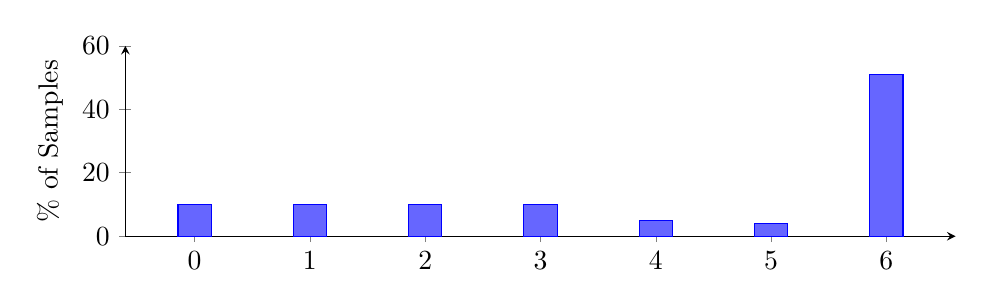
\begin{tikzpicture}
	\begin{axis}[
		width=\textwidth,
		height=4cm,
		ybar,
		bar width=12pt,
		axis x line=bottom,
		axis y line=left,
		ylabel={\% of Samples},
		symbolic x coords={0,1,2,3,4,5,6},
		xtick=data,
%		xticklabel style={rotate=0,anchor=east},
		enlarge x limits=0.1,
		ymin=0, ymax=60
		]
		\addplot+[fill=blue!60] coordinates {
			(0,10) (1,10) (2,10) (3,10) (4,5) (5,4) (6,51)
		};
	\end{axis}
\end{tikzpicture}

  \begin{columns}[t]
	\column{0.33\textwidth}
	\centering\footnotesize
	\begin{tabular}{r l}
		0 & Anger   \\
		1 & Disgust \\
		2 & Fear    
	\end{tabular}
	
	\column{0.33\textwidth}
	\centering\footnotesize
	\begin{tabular}{r l}
		3 & Happy     \\
		4 & Sad       \\
		5 & Surprised 
	\end{tabular}
	
	\column[c]{0.33\textwidth}
	\centering\footnotesize
	\begin{tabular}{r l}
		6 & Neutral\\
		  &  \\
		  &
	\end{tabular}
\end{columns}



			\end{center}
			
		\end{column}
		\begin{column}{0.5\textwidth}
		\centering
		\small
		\begin{tabular}{lcc}
		\toprule
		\textbf{Signal} & \textbf{Rate (Hz)} & \textbf{Channels} \\
		\midrule
		BVP  & 64 & 1      \\
		ACC  & 32 & 3 		\\
		EDA  & 4  & 1      \\
		HR   & 1  & 1      \\
		\bottomrule
		\end{tabular}
		
		\begin{block}{}
			20 970 sensor‐only samples (4 s windows)
		\end{block}

		\end{column}
		
	\end{columns}
\end{frame}


\begin{frame}[t]{Problem Setting}
	\begin{block}{}
		Let $\{(\boldsymbol{x}^{(i)},\,y^{(i)})\}_{i=1}^N$ be the training dataset, where 
		$\boldsymbol{x}^{(i)}\in\mathcal{X}$ and $y^{(i)}\in\{0,1,\dots,6\}$.  
		Here $\mathcal{X}$ is the space of vector sequences of length $T=256$:
		\[
		\boldsymbol{x}^{(i)}
		= \bigl[\boldsymbol{x}^{(i)}_{1}, \dots, \boldsymbol{x}^{(i)}_{t}, \dots,\boldsymbol{x}^{(i)}_{T}\bigr].
		\]
		Each vector $\boldsymbol{x}^{(i)}_{t}$ has $p=6$ elements by channels,
		denoted $x^{(i)}_{t,j}\in\mathbb{R}$ or be a missing value $\hat{x}^{(i)}_{t,j}$.
	\end{block}
	
\begin{center}
	\begin{tikzpicture}[x=1.2cm,y=1.2cm]
		\foreach \i in {0,...,4} {
			\fill[fill=MyAccent!20, draw=MyDarkBlue] (\i,0) rectangle ++(1,1);
			\node[text=MyDarkBlue, font=\footnotesize] at (\i+0.5,0.5) {$x_{\i}$};
		}
	\end{tikzpicture}
\end{center}

\end{frame}


